\section*{Results}

We explored the influences of two internal parameters: $b_3$ (\cref{eq:eg}) which scales the effect of body size on resource allocation and conductance $K_1$ and $K_2$ which defines the passive loss of heat during warm-up, convection, and two environmental variables: environmental temperature $T_e$ and the amount of resource available $R$.

Our main goal is to understand the role of different processes in shaping the energy budget of a species given its body mass

% E: Good strategy to give basics of model behavior first, and then put it together for the more complicated niche questions!

\subsection*{Role of foraging}
The amount of resources an individual acquires can be limited by time (\cref{fig1}a) or by the amount of resources that are available (\cref{fig1}b).

\cref{fig1}a shows how the exponent of the foraging rate influences the net energy gain.
When the exponent $b_3$ is large enough (here 0.8 or 1.25), energy gain increases with body size.
However, when $b_3$ decreases, net energy gain becomes a non-monotonic function of body size.
Net energy gain becomes a decreasing function of body mass for large values because the energetic gain cannot compensate for high energetic costs (demands).
We will explore that fact in more details in the next section, where we also look at the effect of resource availability and quality.     

\cref{fig1}b shows that when resource is limiting, net energy budget decreases with body size (because net energy budget is always zero for an individual of size zero, it has to increase first).
This is expected because large individuals have higher energetic cost.
In this case, the exponent $b_3$ only affects how much the net energy gain decreases with body size. 
When there is enough resource, net energy gain can increase with body size (Supplementary figure). 

\subsection*{When does net energy gain peaks at intermediate body mass?}
Net energy gain only peaks when two conditions  are met (see below for mathematical analysis).
First, $b_3 < b_1 = b_2$ (the equality is by assumption and to reduce the number of free parameter).
% E: so really, the condition is that b_3 is the smallest?
Second, resource quality $\varepsilon$ is within a certain range represented by shades in \cref{fig2}a.
\cref{fig2}a shows for two different temperatures (red = warm, blue = cold) the required values of the resource quality $\varepsilon$ so that net energy gain peaks at intermediate value of body mass.
\cref{fig2}b shows how net energy gain changes as function of body mass for the resource quality shown in \cref{fig2}a.
These conditions are quite restrictive and looks unlikely in real system.
%Given those restrictions, net energy gain will be a monotonic function of body mass.
% E: This is a great example of why it was worth constructing a math model, rather than just intuitive arguments!

In a more technical term, the range of the $\varepsilon$ allowing intermediate optimal body mass is 
\begin{equation}\label{C1}
	\widetilde{E_n} < \varepsilon < \widetilde{dE_n}.
\end{equation}
where,
\begin{flalign*}
\widetilde{E_n} &= \theta_1 + \theta_2, \\
\widetilde{dE_n} &= \frac{b_2}{b_3} \theta_1  +  \frac{b_1}{b_3} \theta_2.
\end{flalign*}
and $$\theta_1 = \frac{a_2}{a_3}  z^{b_2 - b_3}  e^{-E/[k (max(T_w(z_{th}),T_e(t))+ 273.15)]}$$ and $$\theta_2 =  \frac{a_1}{a_3} z^{b_1- b_3}  e^{-E/[k (T_e(t)+ 273.15)]} (\frac{24}{t_f} -1).$$

The difference between  $\widetilde{E_n}$ and  $\widetilde{d E_n}$ is that in  $\widetilde{dE_n}$, each term of  $\widetilde{E_n}$   is weighted by $\frac{b_2}{b_3}$ and $\frac{b_1}{b_3}$.
Thus, a necessary condition for optimal mass to be intermediate (\cref{C1}) is that the weights are larger than 1 i.e.  $b_3 < b_1$ ($b_2 \geq b_1$ is always true). 
As temperature increases, the term with the product $\frac{b_1}{b_3}$ becomes larger thus increasing the range of values where \cref{C1} is true (\cref{fig2}a).

The same reasoning can be used when $E_n$ is a monotonic function of body mass.
If $b_3 > b_2$, $d E_n/dz$ is always positive and $E_n$ becomes an increasing function $z$.
%When $b_1 < b_3 < b_2$, \cref{C1} can still be satisfied but require fine tuning of the remaining parameters. %this is such a special case I rather not explore

\subsection*{Including warm-up.}
Successful warm-up is a necessary condition before foraging. 
It is obvious that under perfect conditions where solar radiation is not limiting and forced convection from wind is absent , any individual can absorb use that energy to warm-up.
We explore here cases where solar radiation is limiting and wind increasing convection between the surface of the individual and the external environment.

\cref{fig3} shows major qualitative outcomes of the minimum temperature required to complete warm-up as a function of body mass.
In \cref{fig3}a, the minimum temperature for warm-up increases with body mass because small individual absorbs more heat (higher surface area-to-body ratio).
This pattern only occurs when the individual relies only solar radiation to warm-up (ectotherm) and there is only free convection (no wind).
In \cref{fig3}b, the minimum temperature for warm-up is lowest at intermediate body size.
This happens because there is now more convection due to wind. 
Small individual are then penalized as convection increases (see \cref{eq:dTr2}).
In \cref{fig3}c, individuals are capable of producing heat endogenously (endotherm).
In this case, the role of surface area-to-body ratio is reversed as the heat generated in the thorax dissipates less with large individuals.
As a consequence, large individual can complete warm-up at lower temperature (\cref{fig3}c).
% E: I repeat my comment above: This is a great example of why it was worth constructing a math model, rather than just intuitive arguments!

\subsubsection*{Duration of warm-up.}
\cref{fig4} shows how long it takes to warm-up as function of how long after sunrise an individual will start.
As expected, duration of warm-up decreases as this intensity of solar radiation increases (it peaks at noon).
The decrease is not linear, warm-up time decreases abruptly and then level off few hours after sunrise (\cref{fig4}a).
For endothermic individual, the same pattern occurs although it is less abrupt compared to ectothermic individuals (\cref{fig4}b) .
For ecothermic individuals, the duration of warm-up increases with body mass (\cref{fig4}a).
For endothermic, it is not necessarily true because the smallest individual can lose too much of the heat it generates to the environment via conductance (\cref{fig4}b).

Conductance between the thorax and the rest-of-the-body plays an important role for the warm-up process and, as expected, has opposing roles for ecotherm and endotherm.
For endotherm, \cref{fig4}c shows how different values for the conductance are favored at different part of the day.
If warm-up is initiated early in the day where solar radiation is weak, low conductance is preferred (thick line \cref{fig4}c).
As the intensity of solar radiation increases, it becomes a dominant source of energy and transferring that energy to the thorax is better achieved with high conductance (dashed line \cref{fig4}c).

\subsection*{Back to the niche}
In \cref{fig5}, we attempt to summarize and integrate all the components above in determining the `niche' of a species.
We focus on three main process: reduction in resource availability, inclusion of warm-up, and change in daily temperature.

\cref{fig5}a shows a default scenario with intermediate resource abundance.
For a range of daily temperature, net energy gain is highest at intermediate body size, large is not optimal for the same reason as in \cref{fig1}b.
As resource abundance decreases, net energy gain decreases dramatically for large individuals (solid lines \cref{fig5}b).
This makes small individual (relatively) more competitive.
Also note that the upper limit of the `niche' is contracted to lower temperature (\cref{fig5}b), simply because the amount of resource available does not compensate the high energetic cost.

When we integrate warm-up processes, which is important when temperature is cold, large individual is also more affected.
Because it takes too much time to warm-up (\cref{fig4}bc).
We assumed here that time spend during warm-up is subtracted in the total time available for foraging.
In short, warm-up contracts the lower part part of the niche.
Supplementary material contains more detailed results where warm-up cannot be completed so that the lower limit will be dictated by the patterns in \cref{fig3}.
% E: discuss endo vs ecto?

Finally, we look at variation in daily temperature.
Instead of having constant daily temperature, we assumed that increases throughout the day.
% E: Wait, so all that above was constant daily temperature?  In that case, maybe don't lead the Methods with variable environmental temperature, or at least explain there that constant is the norm.
This increases in temperature further affects the largest individual (thick line in\cref{fig5}d).
% E: needs more explanation

%
%\subsection*{Net energy budget as a function of body mass: no warm-up}
%We assumed that energy gain always increases with body mass because $b_3$ is always positive (\cref{eq:eg}).
%For fixed environmental temperature, we optimal body size is not necessarily the largest. 
%Large can be suboptimal for two reasons. 
%First, when the exponent for foraging rate (gain) is smaller than exponents of metabolic rate (cost) (\cref{fig1}a, dashed), the gain does not compensate for the loss. 
%The gap increases with body mass (next paragraph for a more detailed analysis). 
%Second, the amount of resource available does not fulfill the energetic demand of large individuals (\cref{fig1}b).
%
%%ADD figure here-ish.
%\begin{figure}
%\begin{center}
%\scalebox{1.5}{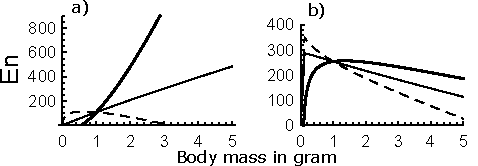
\includegraphics{Fig1}}
%\caption{
%	Daily net energy gain  $E_n$ as function body mass $z$ for $b_2 = 0.5, 0.8, 1.25$, dashed, thin, thick lines, respectively.
%	a) Foraging time $t_f$ is fixed to one hour, b) resource availability $R$ is fixed
%}% Add non trivial units later
%\label{fig1}
%\end{center}
%\end{figure}
%
%Let us return to dashed line in \cref{fig1}a.
%We found that intermediate optimal body mass only occurs under a restricted condition i.e. $d E_n/dz$ is negative for large value of $z$.
%We show the derivation in the supplement but in short we found that resource quality $\varepsilon$ in \cref{eq:eg} needs to be within a certain range (\cref{fig2}a).
%If $\varepsilon$ is too low (\cref{fig2}a, e.g. dashed horizontal line below the red shaded region for $z > 3 $), $E_n$ becomes negative (\cref{fig2}, red dashed).
%If $\varepsilon$ is too high (\cref{fig2}a, e.g. dashed and solid horizontal lines above the blue shaded region),  $d E_n/dz$ becomes positive leading to a monotonic increase in $E_n$ with respect to $z$ (\cref{fig2}b, dashed and solid blue).
%In a more technical term, the range of the $\varepsilon$ allowing intermediate optimal body mass is 
%\begin{equation}\label{C1}
%	\widetilde{E_n} < \varepsilon < \widetilde{dE_n}.
%\end{equation}
%where,
%\begin{flalign*}
%\widetilde{E_n} &= \theta_1 + \theta_2, \\
%\widetilde{dE_n} &= \frac{b_2}{b_3} \theta_1  +  \frac{b_1}{b_3} \theta_2.
%\end{flalign*}
%and $\theta_1 = \frac{a_2}{a_3}  z^{b_2 - b_3}  e^{-E/[k (max(T_w(z_{th}),T_e(t))+ 273.15)]}$ and $\theta_2 =  \frac{a_1}{a_3} z^{b_1- b_3}  e^{-E/[k (T_e(t)+ 273.15)]} (3600 \times24 /t_f -1)$.
%
%The difference between  $\widetilde{E_n}$ and  $\widetilde{d E_n}$ is that in  $\widetilde{dE_n}$, each term of  $\widetilde{E_n}$   is weighted by $\frac{b_2}{b_3}$ and $\frac{b_1}{b_3}$.
%Thus, a sufficient condition for optimal mass to be intermediate (\cref{C1}) is that the weights are larger than 1 i.e.  $b_3 < b_1$ ($b_2 \geq b_1$ is always true). 
%As temperature increases, the term with the product $\frac{b_1}{b_3}$ becomes larger thus increasing the range of values where \cref{C1} is true (\cref{fig2}a).
%The same reasoning can be used in the first paragraph.
%If $b_3 > b_2$, $d E_n/dz$ is always positive and $E_n$ becomes an increasing function $z$.
%When $b_1 < b_3 < b_2$, \cref{C1} can still be satisfied but require fine tuning of the remaining parameters. %this is such a special case I rather not explore
%
%\begin{figure}
%\begin{center}
%\scalebox{1.5}{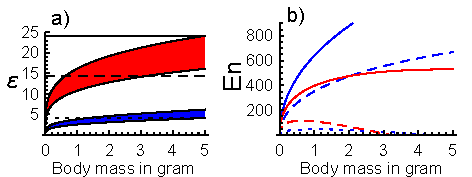
\includegraphics{Fig2}}
%\caption{
%	a) shaded regions show conditions where $E_n$ is maximized at intermediate value of $z$.
%	Resource quality $\varepsilon$ needs to fall inside the shaded regions to satisfy \cref{C1}.
%	The upper (lower) limit of the shade region is $\widetilde{dE_n}$ ($\widetilde{E_n}$).  
%	b) Different shape of $E_n$ based on a).
%	Foraging time $t_f = 1$ hour.
%}% Add non trivial units later
%\label{fig2}
%\end{center}
%\end{figure}
%
%\subsection*{Warm-up}
%\subsubsection*{Ectotherms}
%The ability to warm-up depends on the the surface-to-body ratio.
%Because it decreases with increasing body mass, per unit of mass, smaller individual absorbs more energy that larger ones.
%However, convection decreases with body mass. 
%The effect of these two will generate two patterns.
%\cref{fig3}a shows that for free convection, small can warm-up at lower environmental temperature.
%The largest need higher temperature not only of the smaller surface-to-body ratio but also because their operative temperature $T_w$ is higher.
%\cref{fig3}b shows that when it is windy, warm-up naturally becomes more difficult for any body size.
%The optimal body size for warm-up is generally at intermediate value.
%If the conductance between the rest-of-the-body and the thorax is low, the effect of body size does not dominate and high environmental temperature is required (\cref{fig3}).
%
%\cref{fig4} shows that it usually takes longer for larger body to warm-up (given they can warm-up).
%Evidently, warm-up time is shorter when solar radiation is more intense. 
%Here, the blue and the red denotes warm-up starting at sunrise and three hours after sunrise, respectively. 
%
%\subsection*{Influence of temperature}
%As in \cref{fig1}, the influence of the exponent of the foraging rate $b_3$ and the amount of resource available defines the optimal body mass (\cref{fig5}).
%\cref{fig5}ab show that as long as the exponent $b_3$ is high, large is always optimal.
%However, \cref{fig5}c shows that optimal body mass decreases with increasing temperature when $b_3$ is small.
%When resource is limited, large cannot be advantageous (\cref{fig5} lower panels).
%
%\cref{fig5} assumes that temperature is constant during the day.
%If temperature increases during the day after sunrise, the metabolic costs become higher thus squeeze the thermal niche breadth (defined as the range of temperature with positive net energy gain) to lower value.
%In our model, foraging rate defines the upper thermal breadth.
%
% \subsection*{Combining everything, \cref{fig6,fig7}}
% We summarize here the effects of different components of the model.
% It is important here to note that total foraging time is fixed to 2 hours, thus the longer the warm-up phase, the shorter the time left for foraging.
% One can think of a situation where resources are depleted by the arrival of earlier competitor.  
%  Second, the increment in maximum temperature does not depend on temperature at sunrise. 
%  For instance when temperature at sunrise is 0 (or 20) degree Celsius, then it peaks at 10 (30) degree Celsius at mid-afternoon.
% \begin{itemize}
% 	\item Including warm-up narrows the thermal breadth because
% 	\begin{itemize}
%	 	\item First, warm-up cannot be completed at low temperature preventing foraging.	
%  		\item Second, warm-up takes time and is longer for larger individual (\cref{fig4}. Thus warm-up affects larger individual more and lower thermal breadth is higher for larger individuals
%	\end{itemize}  
%	\item Adding variation in the temperature (incrementation) decreases thermal breadth because metabolic costs increases. 
%	The gain in warm-up ability does not compensate for the increase in energetic cost.
%	\item Increasing $b_3$ favors large individuals thus widens thermal breadth of large individuals and narrows the thermal breadth of small individuals.
%	\item The first strategy to increase thermal breadth is to wait until there is more solar radiation before warming-up.
%	\item The second strategy is to prolong foraging. 
%	This last case of course assumes that resources are not highly limiting.
%\end{itemize}  
%The same pattern is obtained under free or laminar convection. 
%
%\newpage
%\subsection*{Remaining figure captions}
%\begin{figure}[H]
%\begin{center}
%%\scalebox{1.25}{\includegraphics{Fig3}}
%\caption{
%	Minimum environmental temperature required so that warm-up can be completed (maximum time 6 hours).
%	Upper (lower) row represents free (laminar convection).
%	Left (right) is for default (lower) conductance between thorax and the rest-of-the-body ($K_1$ in \cref{eq:dTr1}.
%	Black lines show default value for convection ($K_2$ in \cref{eq:dTr1}), red and blue represent low and convection by one order of magnitude with respect to the default value.
%	Solar radiation was increased gradually from 0 to 1320/4 for 6 hours. 
%	For the laminar convection,  wind speed is (0.5 m/s).
%	Temperature is kept constant
%}% Add non trivial units later
%\label{fig3}
%\end{center}
%\end{figure}
% %   
%\begin{figure}[H]
%\begin{center}
%%\scalebox{1.25}{\includegraphics{Fig4}}
%\caption{
%	Warm-up duration in hour as a function of body size. 
%	Warm-up starting at sunrise (3 hours after sunrise) is denoted by blue (red). 
%	Thin (thick) line represents default (low) conductance ($K_1$) between the thorax and the rest-of-the-body.
%}% Add non trivial units later
%\label{fig4}
%\end{center}
%\end{figure}
%
%\begin{figure}[H]
%\begin{center}
%%\scalebox{1.25}{\includegraphics{Fig5}}
%\caption{
%	Change in net energy gain as a function of constant environmental temperature. 
%	Thick, thin, dashed, gray lines denote respectively an individual with body mass equals to 0.01, 0.1, 1, 5 gram. 
%	Upper row assumes foraging time = 1hour,
%	Lower row assume the total amount of resource available is 5 gram.
%}% Add non trivial units later
%\label{fig5}
%\end{center}
%\end{figure}
%%
%\begin{figure}[H]
%\begin{center}
%%\scalebox{1.25}{\includegraphics{Fig6}}
%\caption{
%	Change in net energy gain as a function of environmental temperature and the marginal effects of different factors under free convection.
%	Line types as in \cref{fig4} except for the thick lines which now represent a body mass of 10 gram.
%	See main text under the section \textbf{Combining everything} for more explanation.
%}% Add non trivial units later
%\label{fig6}
%\end{center}
%\end{figure}
%%
%\begin{figure}[H]
%\begin{center}
%%\scalebox{1.25}{\includegraphics{Fig7}}
%\caption{
%	Same as in \cref{fig6} but under forced convection.
%}% Add non trivial units later
%\label{fig7}
%\end{center}
%\end{figure}
%

%\subsubsection*{Influence of environmental temperature}
%As in the previous section, the results are represented either assuming a fixed foraging time or a fixed amount of resource.
%In the first case, when $b_3$ is large, largest size is optimal for any environmental temperature (\cref{fig3}a).
%However, when $b_3$ is small, optimal body mass is a decreasing function of temperature (\cref{fig3}b).
%%At high temperature, it is easier to satisfy \cref{C1} as it allows a broader range of  resource quality (\cref{fig1}b).
%%note here than in fig1, we changed $\varepsilon$ and in here $varepsilon$ is fixed but the shaded region is low and narrow
%
%Increasing the cost of warm-up does not change the relationship between optimal body mass and temperature but significantly reduces the thermal niche of each individual (\cref{fig3}c).
%However, thermal niche is not only a function of internal parameters, as the quality of resource ameliorates, the thermal niche of the largest individual broadens (\cref{fig3}d).
%
%In the second case where the amount of resource is fixed, intermediate body mass is optimal (\cref{fig3}e). 
%Largest individuals are limited by resource availability and smaller individual cannot gather enough resource due to limited foraging time (we assumed that foraging cannot exceed 12 hours). % not 100% sure..
%Increasing the cost of warm-up penalizes smallest to medium-size individuals such that largest becomes optimal at low temperature (\cref{fig3}f).
%
%As a general conclusion, for all panels in (\cref{fig3}), irrespective of the conditions, optimal environmental temperature decreases with increasing body mass. 
%Depending on parameters $b_3$ and $R$ or foraging time $t_f$, optimal body mass is the largest (\cref{fig2}a), optimal body mass decreases with temperature \cref{fig2}b, or optimal body mass is at intermediate value \cref{fig2}e.
%The capacity of warm-up limits thermal niche of smaller individuals whereas the amount and quality of resource available limits thermal niche of larger individuals.
%
%\begin{figure}
%\begin{center}
%\scalebox{1.25}{\includegraphics{Fig3}}
%\caption{
%	Panels show daily net energy gain  $E_n$ as function of environmental temperature $T_e(t) = \tau$ for 5 body masses.
%	In a), b), c), and d) Foraging time $t_f$ is fixed to one hour.
%	In e) and f) resource availability is $R$ is fixed to 60 g. 
%	In c) resource quality $\varepsilon$ is higher $14.4$, in the remaining panels (a), b), d), e) and f), $\varepsilon = 8.4$.
%	In c), d), and f), conductance is 14 times higher.
%	Other parameters: $a_2 = 10 \times a_1$, remaining parameters as in \cref{fig1}.
%}% Add non trivial units later
%\label{fig3}
%\end{center}
%\end{figure}
%
%
%\subsection*{Result for the warm-up}
%See appendix for preliminary results
%
%\subsection*{Influence of variable environment temperature}
%...
%The main point here is to look at the influence of fluctuating temperature to make the model results more realistic.



%%Don't read this, I kept in case some recycling is required 
%\subsubsection*{Case 1 = No warm-up}
%For simplicity let us assume that there is no need to warm-up so that $e_w = 0 $ and $t_w =  0$.
%\begin{flalign*}
%	e_r(z) & = \varepsilon a_3 z^{b_3} \times t_f  - \left( \rho a_1 z^{b_2} E_0 Q_{10}^{\frac{\tau}{10}} \times t_f +  a_1 z^{b_1} E_0 Q_{10}^{\frac{\tau}{10}}\times (3600\times24 - t_f) \right) \\
%			& =  z_3^{b_3} \left[  \varepsilon a_3 \times t_f  - \rho a_1  E_0 Q_{10}^{\frac{\tau}{10}} z^{b_2 - b_3} \times t_f -  a_1 z^{b_1- b_3}  E_0 Q_{10}^{\frac{\tau}{10}}\times (3600\times24 - t_f) \right] 
%%			& =  z_3^{b_3} \left[  (\varepsilon a_3  - \rho a_1 Q_{10}^{\frac{\tau}{10}} z^{b_2 - b_3}) \times t_f -  a_1 z^{b_1- b_3} Q_{10}^{\frac{\tau}{10}}\times (3600\times24 - t_f) \right] 
%\end{flalign*}
%Thus, the net energy gain is positive if the term between the square brackets is positive, 
%\begin{equation} \label{eq:C1}
%	\frac{\varepsilon a_3}{ E_0 Q_{10}^{\frac{\tau}{10}}} > \rho a_1  z^{b_2 - b_3} +  a_1 z^{b_1- b_3}  (3600 \times24 /t_f -1)
%\end{equation}
%Net energy gain ($e_r$) increases with body size if $\frac{d e_r}{dz} > 0$, i.e. 
%\begin{equation} \label{eq:C2}
%	\frac{\varepsilon a_3}{ E_0 Q_{10}^{\frac{\tau}{10}}} > \rho a_1  z^{b_2 - b_3} \frac{b_2}{b_3} +  a_1 z^{b_1- b_3}  (3600 \times24 /t_f -1) \frac{b_1}{b_3}.
%\end{equation}
%In contrast, net energy gain ($e_r$) decreases with body size if $\frac{d e_r}{dz} <  0$, i.e. 
%\begin{equation} \label{eq:C3}
%	\frac{\varepsilon a_3}{ E_0 Q_{10}^{\frac{\tau}{10}}} < \rho a_1  z^{b_2 - b_3} \frac{b_2}{b_3} +  a_1 z^{b_1- b_3}  (3600 \times24 /t_f -1) \frac{b_1}{b_3}.
%\end{equation}
%% E: Explain why this situation is of particular interest.  absolute vs proportional/specific energy gain
%Inequations~(\ref{eq:C1}) and~(\ref{eq:C3}) give
%\begin{equation} \label{eq:C4}
%	\rho a_1  z^{b_2 - b_3} +  a_1 z^{b_1- b_3}  (3600 \times24 /t_f -1) < \frac{\varepsilon a_3}{ E_0 Q_{10}^{\tau/10}} < \rho a_1  z^{b_2 - b_3} \frac{b_2}{b_3} +  a_1 z^{b_1- b_3}  (3600 \times24 /t_f -1) \frac{b_1}{b_3},
%\end{equation}
%which is true if $b_2 > b_1 > b_3$ and the middle term is fine tuned.
%Thus, smaller individual may gain more energy than large individuals but under rather restricted conditions.
%If $b_3 > b_2 > b_1$,~(\ref{eq:C1}) implies~(\ref{eq:C2}) and net energy gain increases with body size.
%

